\section[Interfaz OSC]{\textit{Output Channels}}
\sectionmark{\textit{Output Channels}}
\label{sec:output_channels}

\subsection{Los parámetros del módulo}

\begin{description}
	\item[Filter] Colorea el sonido hacia grave o el agudo, a modo de combinación de un filtro paso de altos y otro paso de bajos. Solo funciona cuando está conectado hacia el exterior.
	\item[Pan] Paneo del sonido. Funciona para los puertos \textit{stereo} que combinan a los canales del 1 al 4 y del 5 al 8.
	\item[Off] Interruptor que activa y desactiva la salida del canal hacia los puertos del sintetizador. Cuando está \textit{Off}, el canal puede seguir siendo utilizado a modo de \textit{bus}.
	\item[Level] Ganancia de salida del canal. Solo tiene efecto hacia los puertos del sintetizador.
\end{description}

\begin{figure}
	\centering
	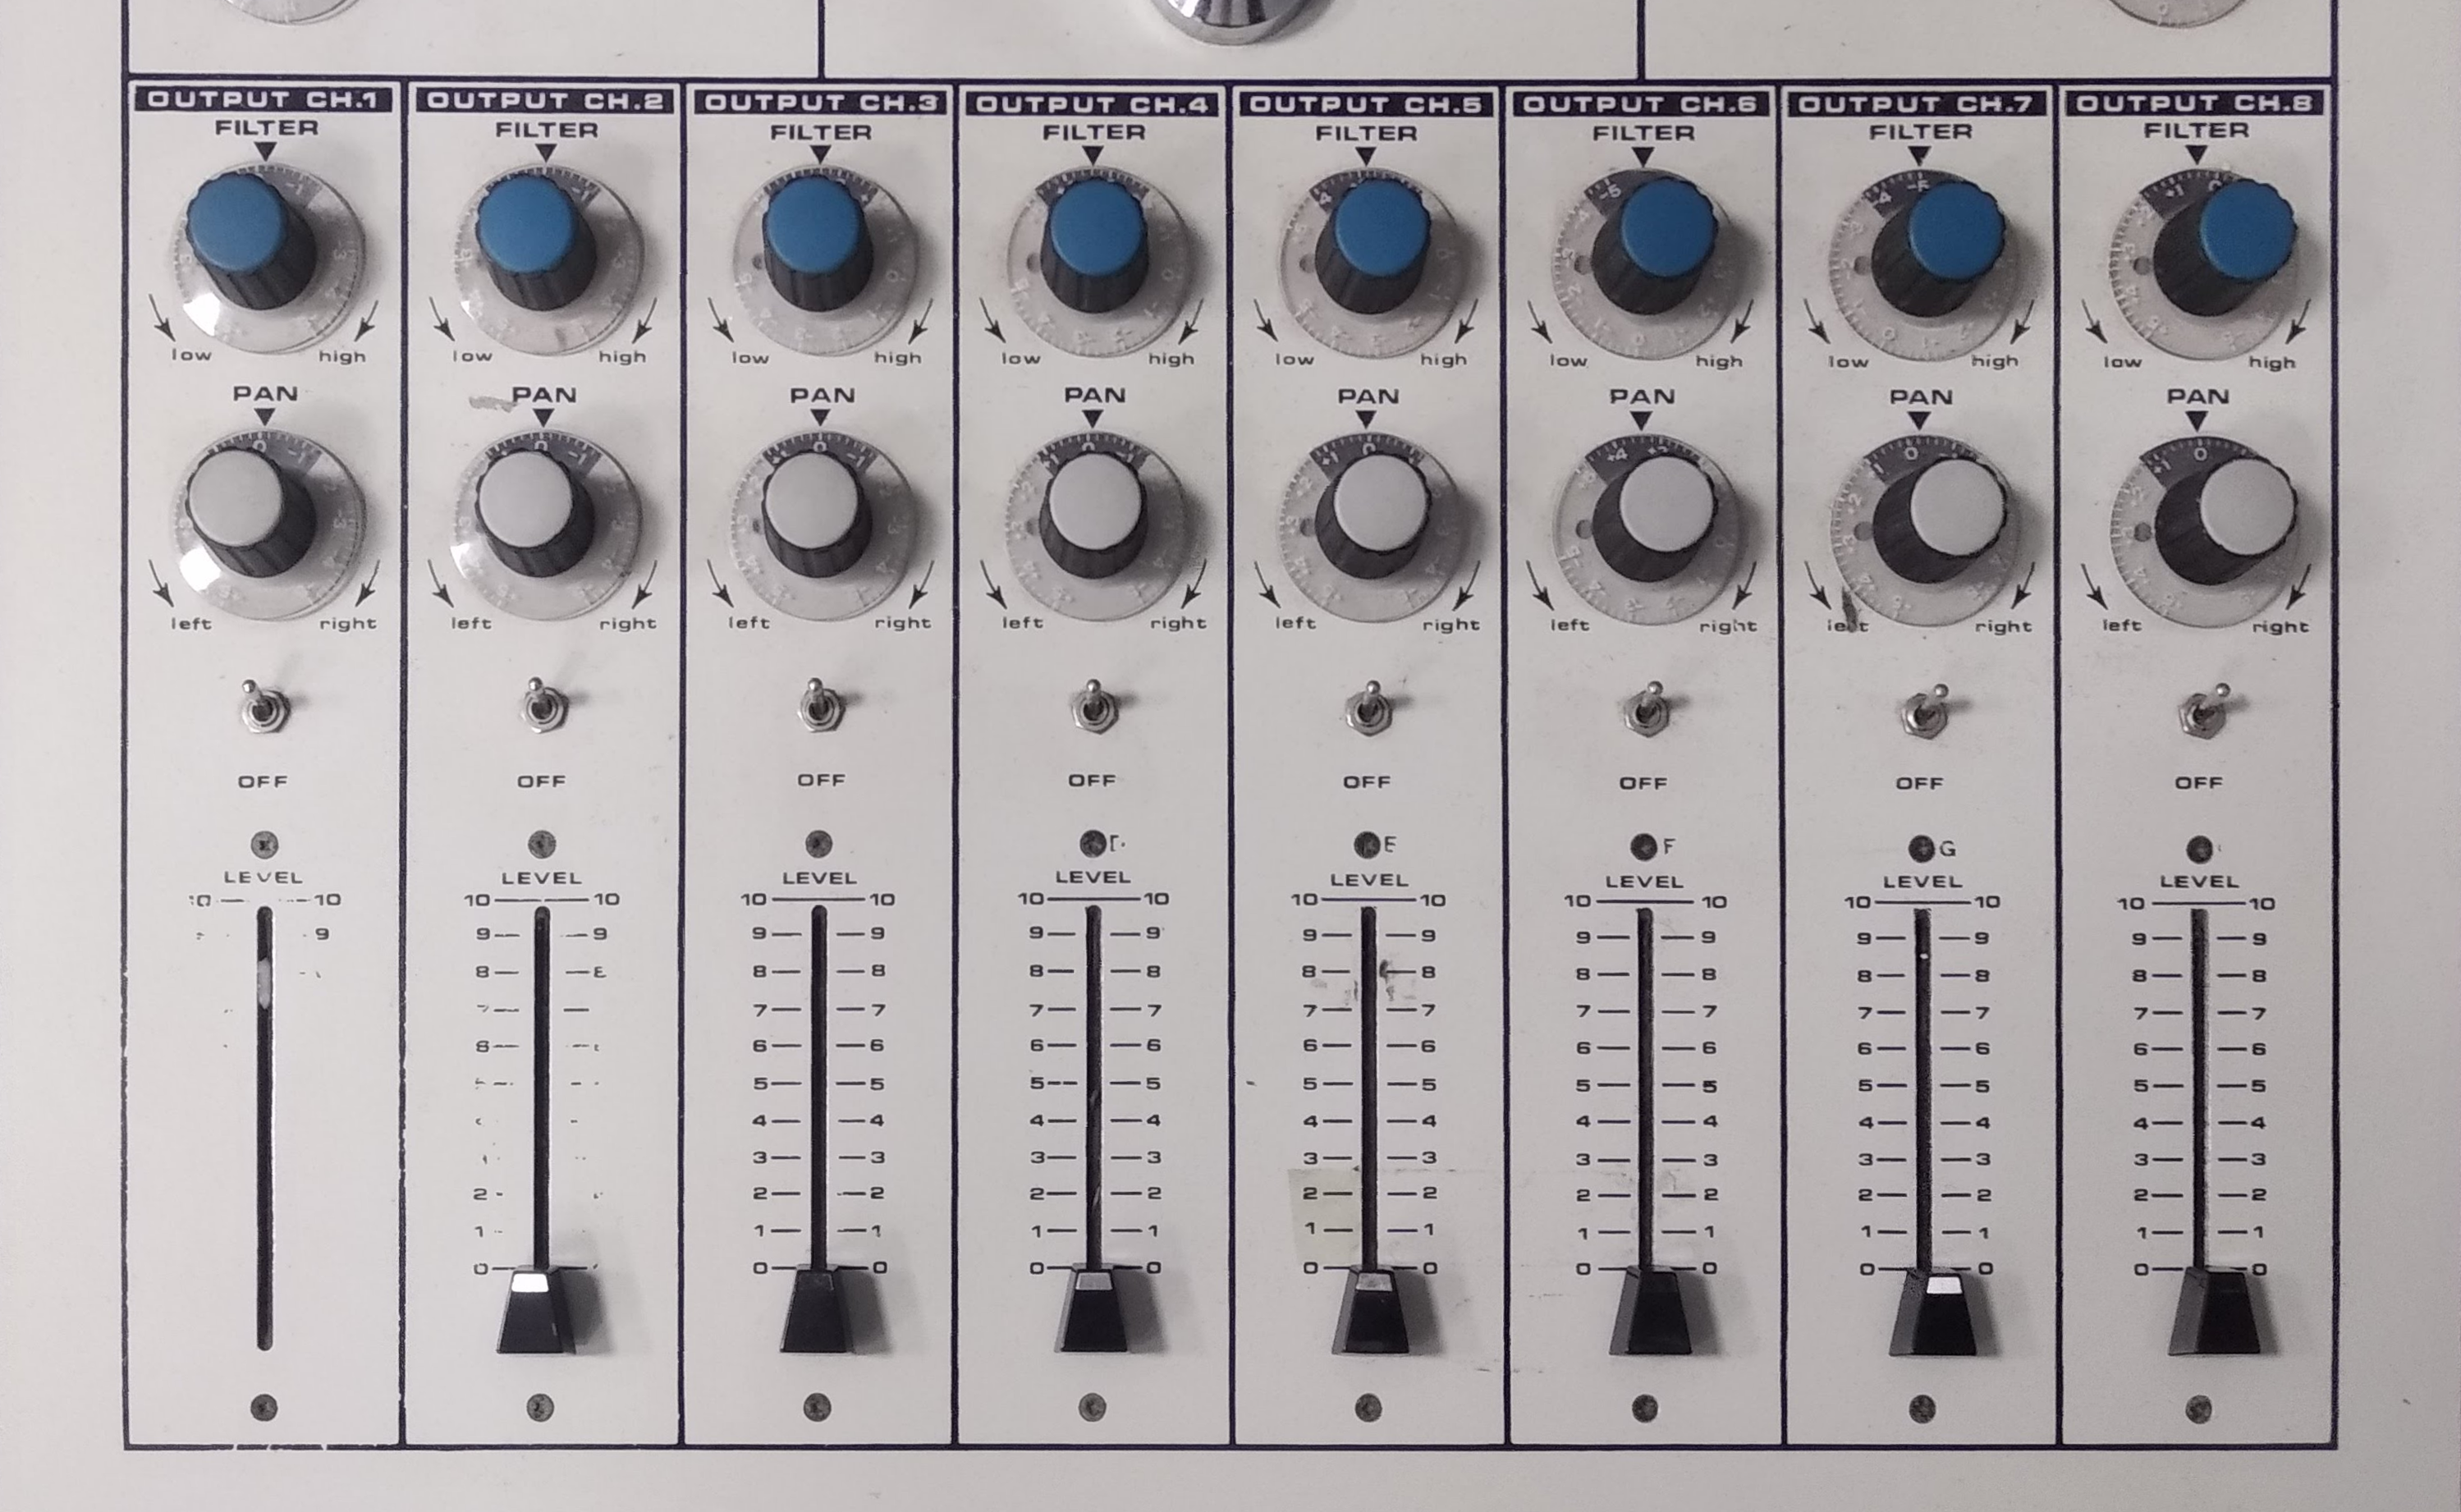
\includegraphics[width=0.7\textwidth]{images/output_channels}
	\caption[\textit{Output Channels}]{Vista del módulo \textit{Output Channels}, 8 canales de salida independientes. Se aprecia en la foto el estado del Synthi 100 del GME, al que le falta uno de los controles deslizantes debido al repetido uso del mismo.}
	\label{fig:output_channels}
\end{figure}